\documentclass[11pt,letterpaper]{article}
\usepackage[
    lmargin=2.2in,
    rmargin=0.7in,
    tmargin=1.0in,
    bmargin=1.0in
]{geometry}
\usepackage{notes}
\usetikzlibrary{arrows.meta,decorations.markings}
\usepackage{pgfplots}
\pgfplotsset{compat=1.18}


% Shared figure styles. Arrows on trajectories always show increasing time.
\definecolor{curve}{HTML}{247E91}
\tikzset{
    orbit/.style={black,thick},
    inward/.style={blue,very thick},
    outward/.style={red,very thick}
}
\newcommand{\phaseaxes}{%
    \draw[->,gray](-3.25,0)--(3.45,0)node[right]{$x$};
    \draw[->,gray](0,-3.25)--(0,3.45)node[above]{$y$};
}
\newcommand{\saddlerays}{%
    \draw[outward](-3.1,0)--(3.1,0);
    \draw[inward](0,-3.1)--(0,3.1);
    \foreach \s in {-1,1}{
        \draw[->,outward](.9*\s,0)--(1.7*\s,0);
        \draw[->,inward](0,1.7*\s)--(0,.9*\s);
    }
    \fill(0,0)circle(2pt);
}
\newcommand{\saddlecurves}{%
    \foreach \sx in {-1,1}{\foreach \sy in {-1,1}{\foreach \c in {.6,1.4}{
        \pgfmathsetmacro{\startx}{(\c/3.1)^2}
        \draw[orbit]plot[domain=\startx:3.1,samples=120]
            ({\sx*\x},{\sy*\c/sqrt(\x)});
        \draw[->,orbit]plot[domain=.85:1.2,samples=20]
            ({\sx*\x},{\sy*\c/sqrt(\x)});
    }}}
}
\newcommand{\velocityfield}{%
    \foreach \xx in {-3,-2,-1,0,1,2,3}{\foreach \yy in {-3,-2,-1,0,1,2,3}{
        \pgfmathsetmacro{\mag}{sqrt(4*\xx*\xx+\yy*\yy)}
        \ifdim\mag pt>0pt
            \draw[->,gray!65](\xx,\yy)--
                ({\xx+.4*2*\xx/\mag},{\yy-.4*\yy/\mag});
        \fi
    }}
}
% Argument -1 gives inward motion, +1 outward motion.
\newcommand{\noderays}[1]{%
    \ifnum#1<0\def\raystyle{inward}\else\def\raystyle{outward}\fi
    \draw[\raystyle](-3.1,0)--(3.1,0);
    \draw[\raystyle](0,-3.1)--(0,3.1);
    \foreach \s in {-1,1}{
        \draw[->,\raystyle]({\s*(1.3-.4*#1)},0)--({\s*(1.3+.4*#1)},0);
        \draw[->,\raystyle](0,{\s*(1.3-.4*#1)})--(0,{\s*(1.3+.4*#1)});
    }
    \fill(0,0)circle(2pt);
}
\newcommand{\nodecurves}[1]{%
    \foreach \sx in {-1,1}{\foreach \c in {-.9,-.25,.25,.9}{
        \pgfmathsetmacro{\endx}{min(3.1,sqrt(3.1/abs(\c)))}
        \draw[orbit]plot[domain=.02:\endx,samples=100]({\sx*\x},{\c*\x*\x});
        \pgfmathsetmacro{\fromx}{1-.18*#1}
        \pgfmathsetmacro{\tox}{1+.18*#1}
        \draw[->,orbit]plot[domain=\fromx:\tox,samples=20]({\sx*\x},{\c*\x*\x});
    }}
}

\begin{document}
\begin{center}\Large\textbf{DAY 31 -- Phase Portraits: Linear Orbits, Saddles, and Nodes}\\
\normalsize (Section 4.4.1)\end{center}


%%%%%%%%%%%%%%%%%%%%%%%%%%%%%%%%%%%%%%%%%%%%
\section{Phase Portraits}

% SIDE NOTE: 9:00 | Goal
% a) One IC: one solution.
% b) Sketch its trajectory.
% c) Different ICs: more trajectories.

Last time, we learned to solve $\mathbf{x}'=A\mathbf{x}$.
Today, we will sketch the straight trajectories first, then use them
to understand the curved trajectories between them.

%-------------------------------------------------------------
\subsection{Phase Plane}

We are interested in the \textit{family of solutions}
to the system
\[
    \mathbf{x}'=A\mathbf{x}.
\]
If $A$ has two distinct real eigenvalues, the general
solution is
\begin{equation}    \label{1}
    \mathbf{x}(t)
    =c_1e^{\lambda_1t}\mathbf{v}_1
    +c_2e^{\lambda_2t}\mathbf{v}_2,
\end{equation}
where $\mathbf{v}_1$ and $\mathbf{v}_2$ are eigenvectors
corresponding to $\lambda_1$ and $\lambda_2$.
Different choices of $c_1$ and $c_2$ give different
members of this family. Each solution $\mathbf{x}(t)=(x(t),y(t))$
traces a \textit{trajectory} when plotted parametrically
in the $xy$-plane. In this setting, we call the
$xy$-plane the \textbf{phase plane}.
The axes represent $x$ and $y$; time is not an axis.

An important property is that \textbf{distinct trajectories
cannot intersect}. It is possible for two solutions to have identical trajectories. If two trajectories are not identical, they will never share a common point.

%-------------------------------------------------------------
\subsection{Initial Condition}

An \textbf{initial condition}
\[
    \mathbf{x}(0)=
    \begin{pmatrix}x_0\\y_0\end{pmatrix}
\]
determines the constants $c_1$ and $c_2$.
Since both exponential factors equal $1$ at $t=0$, combining equation \eqref{1} with the IC yields
\[
    c_1\mathbf{v}_1+c_2\mathbf{v}_2
    =\begin{pmatrix}x_0\\y_0\end{pmatrix}.
\]
This selects one member of the family.
An important property is that \textbf{its trajectory passes through the coordinate}
$(x_0,y_0)$ on the phase plane.

%-------------------------------------------------------------

\subsection{Diagonal Matrices}

Our first example has a \textit{diagonal matrix}. A matrix is called \textbf{diagonal}
if the top-right and bottom-left entries are zero:
\[
    A=
    \begin{pmatrix}
        \alpha&0\\
        0&\beta
    \end{pmatrix}.
\]
Diagonal matrices are convenient because they have simple eigenvalues and eigenvectors:
\[
    \lambda_1=\alpha,\qquad
    \mathbf{v}_1=\begin{pmatrix}1\\0\end{pmatrix},
    \qquad
    \lambda_2=\beta,\qquad
    \mathbf{v}_2=\begin{pmatrix}0\\1\end{pmatrix}.
\]
As an exercise, you should verify this. 

%-------------------------------------------------------------

\begin{example}[1]{
Find the solution to 
\[
\mathbf{x}'=\begin{pmatrix}2&0\\0&-1\end{pmatrix}\mathbf{x},\qquad
\mathbf{x}(0)=\begin{pmatrix}1\\0\end{pmatrix}.
\]
Then plot its trajectory on the phase plane.
}

Since $A$ is diagonal, the eigenvalues are simply $\lambda_1=2$ and $\lambda_2=-1$ with corresponding eigenvectors $\textbf{v}_1=(1,0)$ and $\textbf{v}_2=(0,1)$. The general solution is
\[
\mathbf{x}(t)=c_1e^{2t}\begin{pmatrix}1\\0\end{pmatrix}
+c_2e^{-t}\begin{pmatrix}0\\1\end{pmatrix}.
\]
Applying the initial condition gives us the solution
\[
\begin{pmatrix}c_1\\0
\end{pmatrix} + \begin{pmatrix}
    0\\c_2
\end{pmatrix} = \begin{pmatrix}
    1\\0
\end{pmatrix}
\implies 
\mathbf{x}(t)=\begin{pmatrix}e^{2t}\\0\end{pmatrix}.
\]
Since $x(t)>0$ and $y(t)=0$, the trajectory is the positive $x$-axis, excluding the origin. As $t$ increases, the particle moves to the right. As $t\to-\infty$ approaches $x\to 0$, the trajectory traces back to the origin. Notice that the trajectory passes through the point $(1,0)$.

\begin{center}
\begin{tikzpicture}[scale=.7]
\draw[->,gray](-.6,0)--(4.4,0)node[right]{$x$};
\draw[->,gray](0,-.5)--(0,1)node[above]{$y$};
\draw[red,thick](0,0)--(4,0);
\draw[->,red,thick](1.5,0)--(2.5,0);
\draw[fill=white,red](0,0)circle(2pt);\fill(1,0)circle(2pt)node[below]{$(1,0)$};
\end{tikzpicture}\end{center}
\end{example}

% ---------------------

\subsection{More Initial Conditions}
We can repeat Example 1 with a few other initial conditions: 
$$
\begin{pmatrix}
    -2\\0
\end{pmatrix},\quad 
\begin{pmatrix}
    0\\2
\end{pmatrix},\quad 
\begin{pmatrix}
    0\\-0.5
\end{pmatrix}.\quad 
$$
If we solve the IVP for each IC and plot the trajectories all on the same phase plane, we obtain the following graph on the left. 
\begin{center}
\begin{minipage}[t]{.40\linewidth}\centering
\resizebox{.8\linewidth}{!}{
\begin{tikzpicture}[>=Stealth]
\phaseaxes\saddlerays
\draw[fill=white,red](0,0)circle(2pt);\fill(1,0)circle(2pt)node[below]{$(1,0)$};
\fill(-2,0)circle(2pt)node[below]{$(-2,0)$};
\fill(0,2)circle(2pt)node[right]{$(0,2)$};
\fill(0,-0.5)circle(2pt)node[below left]{$(0,-0.5)$};
\end{tikzpicture}
}

\small Four trajectories
\end{minipage}\hfill
\begin{minipage}[t]{.40\linewidth}\centering
\resizebox{.80\linewidth}{!}{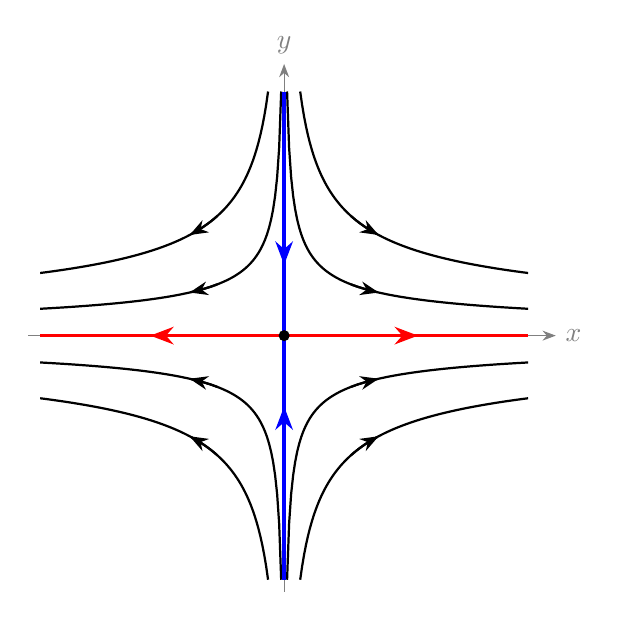
\begin{tikzpicture}[>=Stealth]
\phaseaxes\saddlecurves\saddlerays
\end{tikzpicture}}

\small A phase portrait
\end{minipage}
\end{center}

% ---------------------
\subsection{Goal}
Our goal is to learn how to sketch \textit{phase portraits}. A \textbf{phase portrait} is a sketch that shows multiple solution curves for a system $\textbf{x}'=A\textbf{x}$ on a single phase plane. An example is shown in the figure above on the right. 

Phase portraits are not meant to be perfectly accurate drawings. They are qualitative tools that paint a picture of the possible dynamics that a system may exhibit. You will learn how to sketch phase portraits based on eigenvalues and certain rules about the classification of the phase portrait.

%%%%%%%%%%%%%%%%%%%%%%%%%%%%%%%%%%%%%%%%%%%%%%%%%%%%%%%%%%%%%%%%%%%%%%%%
\section{Equilibria and Direction Fields}

% SIDE NOTE: 9:08 | Recall the 1D picture
% a) Equilibria divide the phase line into intervals.
% b) Signs tell us the direction of motion.
% c) Today: use special trajectories to organize the phase plane.
\subsection{Recall Autonomous Equations}
For the \textit{autonomous equation} $x'=x(1-x)$, we found the equilibria $x=0$ and
$x=1$. These points divided the phase line into intervals. The sign of $x'$
told us whether solutions increased or decreased in each interval. We then used that information to sketch solution graphs in the $tx$-plane. The system $\textbf{x}'=A\textbf{x}$ is a 2D autonomous equation, so many concepts carry over.

Today, we use a similar idea in two dimensions: identify simple parts of the
picture, then determine the motion between them. Our phase portraits are
in the $xy$-plane, with time represented by arrows.

\subsection{Equilibrium Solutions}
An \textbf{equilibrium solution} to $\textbf{x}'=A\textbf{x}$ is a constant solution
$\mathbf{x}(t)=\mathbf{x}^*$. Since its derivative is zero, you may find $\textbf{x}^*$ by solving
\[
    \boxed{A\mathbf{x}^*=\mathbf0.}
\]
Notice that the origin $\textbf{x}^*=(0,0)$ is always an equilibrium. If $\det(A)\ne0$, it is the only one. We mark it with a point, without a motion arrow. 

Graphically, the equilibrium $\textbf{x}^*$ is just a point on the phase portrait. It is the central focus of phase portraits. The family of trajectories have a certain structure that revolves around the equilibrium.

% SIDE NOTE: Direction field -- brief preview
% a) A x is the velocity at x.
% b) Calculate only the arrow at (1,1).
% c) Do not construct the whole field by hand.
\subsection{Direction Fields}
At a point $\mathbf{x}$, the vector $A\mathbf{x}$ gives the
\textbf{velocity vector}. A \textbf{direction field} displays these directions
at many points. Solution trajectories follow the arrows.

For example, at $(1,1)$ in the system from Example 1,
\[
\mathbf{x}'=
\begin{pmatrix}2&0\\0&-1\end{pmatrix}\begin{pmatrix}1\\1\end{pmatrix}
=\begin{pmatrix}2\\-1\end{pmatrix}.
\]
The particle moves right and down. Place the arrow's tail at $(1,1)$.
\begin{center}
\begin{minipage}[t]{.47\linewidth}\centering
\resizebox{.9\linewidth}{!}{\begin{tikzpicture}[>=Stealth]
\phaseaxes\velocityfield
\fill(1,1)circle(2pt);
\draw[->,purple,very thick](1,1)--(1.8,.6);
\node[above right,purple]at(1,1){$(1,1)$};\fill(0,0)circle(2pt);
\end{tikzpicture}}

\small A direction field.
\end{minipage}\hfill
\begin{minipage}[t]{.47\linewidth}\centering
\resizebox{.9\linewidth}{!}{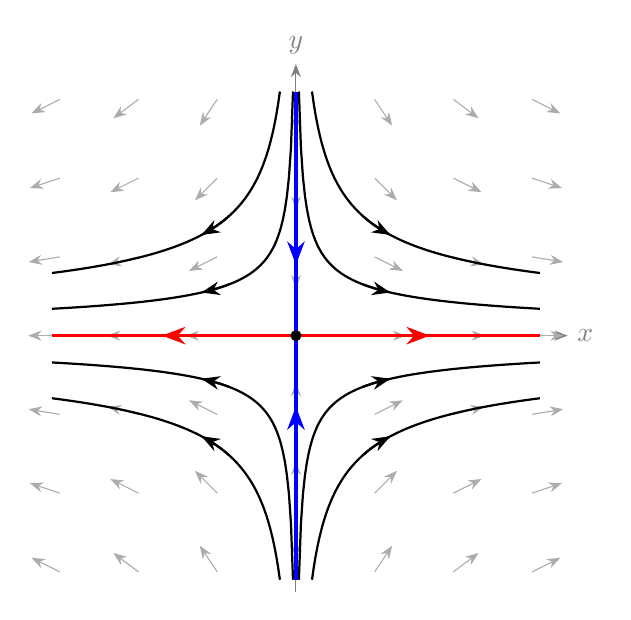
\begin{tikzpicture}[>=Stealth]
\phaseaxes\velocityfield\saddlecurves\saddlerays
\end{tikzpicture}}

\small Trajectories follow the field.
\end{minipage}
\end{center}
You will not need to draw an entire direction field by hand. We will use
linear orbits to guide our sketches, along with a velocity arrow when useful.

%%%%%%%%%%%%%%%%%%%%%%%%%%%%%%%%%%%%%%%%%%%%%%%%%%%%%%%%%%%%%%%%%%%%%%%%
\section{Linear Orbits}

% SIDE NOTE: 9:12 | Main idea
% a) Set c2=0, then set c1=0.
% b) Each eigenvector line gives two rays.
% Ask: if c changes sign, does inward motion become outward? No.
% c) Distinguish the sum of solutions from the union of their paths.
\subsection{Four Rays}
Suppose $A$ has two distinct, real, nonzero eigenvalues. Its general solution is
\[
\mathbf{x}(t)=c_1e^{\lambda_1t}\mathbf v_1+c_2e^{\lambda_2t}\mathbf v_2.
\]
By setting either $c_2=0$ or $c_1=0$, we to obtain one of two \textbf{linear orbits}
$$
\mathbf{x}_1(t)=c_1e^{\lambda_1t}\mathbf v_1 \quad\text{ or }\quad 
\mathbf{x}_2(t)=c_2e^{\lambda_2t}\mathbf v_2
$$
Recall that linear orbits trace out a \textit{ray} in the phase plane. The rays may point toward the origin or off to infinity.

The constant coefficients $c_1$ and $c_2$ can be positive or negative, which can flip the direction of the rays. 
Because there are \textbf{two linear orbits} with arbitrary constants, we have a total of \textbf{four rays} altogether. The first step is to plot the four rays. Let's return to our diagonal example.

\begin{example}[2]{
Sketch the linear orbits for 
\[
\mathbf{x}(t)=c_1e^{2t}\begin{pmatrix}1\\0\end{pmatrix}
+c_2e^{-t}\begin{pmatrix}0\\1\end{pmatrix}.
\]
}
\paragraph{Step 1. Draw the first eigenvector line.}
The vectors $\pm(1,0)^T$ lie on the $x$-axis. Draw the line through them.
Since 
$\lim_{t\to\infty} e^{2t}=\infty$
both rays point away from the origin: right on the positive ray and left on the negative ray.

\paragraph{Step 2. Draw the second eigenvector line.}
The vectors $\pm(0,1)^T$ lie on the $y$-axis. Since
$\lim_{t\to\infty} e^{-t}=0$
both rays point toward the origin: down on the positive ray and up on the negative ray.

\begin{center}
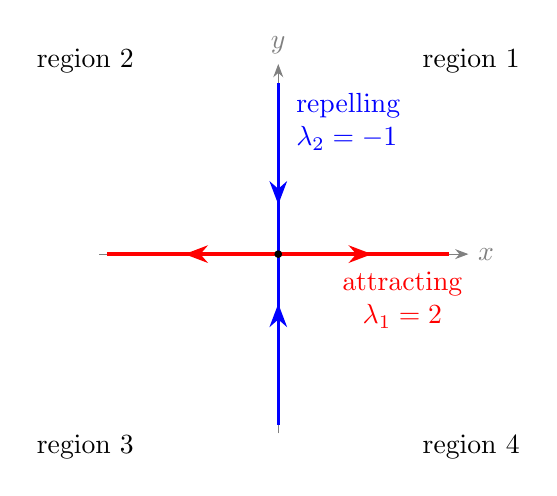
\begin{tikzpicture}[scale=.7,>=Stealth]
\phaseaxes\saddlerays
\node[red,below,align=center]at(2.25,-.15){attracting\\$\lambda_1=2$};
\node[blue,right,align=left]at(.15,2.4){repelling\\$\lambda_2=-1$};
\node at (3.5,3.5) {region 1};
\node at (-3.5,3.5) {region 2};
\node at (-3.5,-3.5) {region 3};
\node at (3.5,-3.5) {region 4};
\end{tikzpicture}
\end{center}
\end{example}

\subsection{Attracting versus Repelling}
The sign of $\lambda$ determines whether the rays of a linear orbit point in or out
\[
\boxed{
\lambda>0:\ \text{rays point away from the origin},\qquad
\lambda<0:\ \text{rays point toward the origin}.
}
\]
We can think of this as a property of the equilibrium point. Along one direction, the point $\textbf{x}^*$ repels nearby solution curves. Along the other direction, the point $\textbf{x}^*$ attracts nearby solution curves. This is related to a concept called \textit{stability}. This is very similar to the way we classified equilibria for 1D autonomous equations. 


\subsection{What Happens Between the Lines?}
The two eigenvector lines divide the plane into four \textit{regions}.
There are solution curves that exist in these regions. What do they look like?
No two trajectories on a phase plane are allowed to intersect. This means that
\textbf{solution curves are restricted to one region}.

%%%%%%%%%%%%%%%%%%%%%%%%%%%%%%%%%%%%%%%%%%%%%%%%%%%%%%%%%%%%%%%%%%%%%%%%
\section{The Saddle Node}

% SIDE NOTE: 9:21 | One curve, then the family
% a) Start at (1,1).
% b) Eliminate t and determine orientation.
% c) Keep each curve inside its region.
\subsection{One Representative Trajectory}
The trajectories in each region all behave according to a certain pattern. We can choose any initial condition in one of the four regions. For simplicity, we will use $\textbf{x}_0=(1,1)$ in region 1 as the initial condition and then plot it.

\begin{example}[3]{
Find the solution to 
\[
\mathbf{x}'=\begin{pmatrix}2&0\\0&-1\end{pmatrix}\mathbf{x},\qquad
\mathbf{x}(0)=\begin{pmatrix}1\\1\end{pmatrix}.
\]
Then plot its trajectory on the phase plane.
}
\paragraph{Step 1. Apply the initial condition.}
At $t=0$, we obtain $c_1=c_2=1$. Therefore,
\[
x(t)=e^{2t},\qquad y(t)=e^{-t}.
\]
\paragraph{Step 2. Find the shape.}
Since $\sqrt{x}=e^t$, we can eliminate $t$ by substituting it into  $y=(e^{t})^{-1}$:
\[
\boxed{y=\frac{1}{\sqrt{x}},\qquad x>0.}
\]
\paragraph{Step 3. Determine orientation and limits.}
As $t$ increases, $x$ increases and $y$ decreases. The particle moves
right and down through $(1,1)$, consistent with the velocity $(2,-1)^T$.
\[
\begin{array}{c|cc}
 & x(t)&y(t)\\\hline
 t\to-\infty&0&+\infty\\
 t\to+\infty&+\infty&0
\end{array}
\]
The curve comes in close to the inward ray, bends, and heads out close to
the outward ray. It never crosses either axis or reaches the origin.
\begin{center}
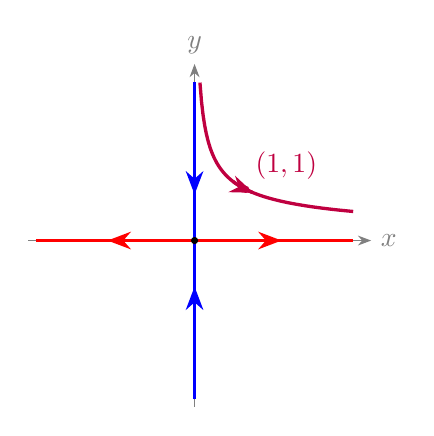
\begin{tikzpicture}[scale=.65,>=Stealth]
\phaseaxes\saddlerays
\draw[purple,very thick]plot[domain=.105:3.1,samples=100](\x,{1/sqrt(\x)});
\draw[->,purple,very thick]plot[domain=.75:1.15,samples=20](\x,{1/sqrt(\x)});
\fill[purple](1,1)circle(2pt)node[above right]{$(1,1)$};
\end{tikzpicture}
\end{center}
\end{example}

\subsection{Classification and Terminology}

\cols{
For this diagonal system, every curved trajectory has the form
\[
 y=\frac{C}{\sqrt{|x|}},\qquad C\ne0,
\]
on either $x>0$ or $x<0$. The constant $C$ selects the height and sign
of the curve. Draw one or two representative curves in each region. The curves move in along the attracting ray then bend out along the repelling ray. Then we have a complete phase portrait, as shown in the figure to the right.
}{
\begin{center}
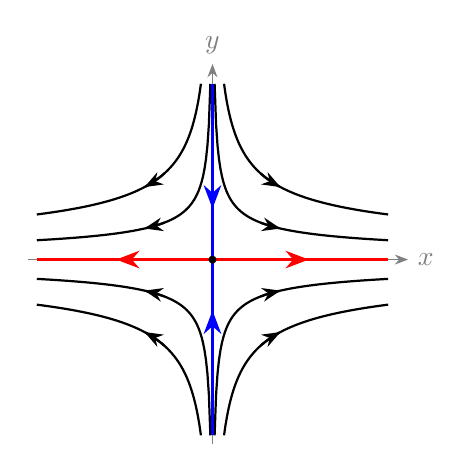
\begin{tikzpicture}[scale=.72,>=Stealth]
\phaseaxes\saddlecurves\saddlerays
\end{tikzpicture}
\end{center}
}



The equilibrium point $\textbf{x}^*=(0,0)$ is an important part of phase portraits. They can be classified as one of 7 types. When the eigenvalues of $A$ are real and have opposite signs, we say that $\textbf{x}^*$ is a \textbf{saddle node}. 

The shape of this phase portrait is called a \textbf{saddle structure}. Whenever you have opposite-sign real eigenvalues, the phase portrait will have this similar overall shape. The trajectories are not exactly hyperbolas. The curves are "hyperbola-like" in the sense that the trajectories head toward the origin and then bend away. We will see this in the next saddle example.


\subsection{A Saddle with Tilted Eigenvector Lines}
The same approach works when the eigenvectors do not lie on the coordinate axes.
The regions are then the sectors between the eigenvector lines, not necessarily
the four coordinate quadrants. Draw the linear orbits. Then draw curved trajectories in each of the four regions that move toward the equilibrium and bend away.

% SIDE NOTE: 9:29 | Transfer the method
% a) Draw lines and orient all four rays.
% b) Add curves without crossing the lines.
% c) Mark (2,2); exact constants are optional.
% If behind, omit the highlighted initial-point discussion and start nodes at 9:36.
\begin{example}[4]{
Sketch the phase portrait for
\[
\mathbf{x}(t)=c_1e^{2t}\begin{pmatrix}1\\3\end{pmatrix}
+c_2e^{-t}\begin{pmatrix}2\\-1\end{pmatrix}.
\]
Mark the trajectory through $(2,2)$.
}
\paragraph{Step 1. Draw and orient the linear orbits.} You know how to sketch unshifted rays. The eigenvectors determines the direction and the eigenvalue determines the orientation.  
\[
\begin{array}{c|c|c}
\text{Eigenvector}&\text{Line}&\text{Orientation}\\\hline
(1,3)^T&y=3x&\lambda_1=2:\ \text{outward (repelling)}\\
(2,-1)^T&y=-x/2&\lambda_2=-1:\ \text{inward (attracting)} 
\end{array}
\]
\paragraph{Step 2. Add curves in each region.}
Draw curves coming in towards the origin along the attracting ray, and bending away along the neighboring repelling ray. Keep each curve in its region. Do not intersect trajectories.

The exponentials explain the motion: as $t$ increases, $e^{-t}$ decays
and $e^{2t}$ grows. Eventually, the trajectory heads outward in the
direction determined by the $\mathbf v_1$ term.

\paragraph{Step 3. Mark the initial point.}
Plot $(2,2)$ and draw a curve through it in its region. A qualitative sketch
does not require solving for $c_1$ and $c_2$.

\begin{center}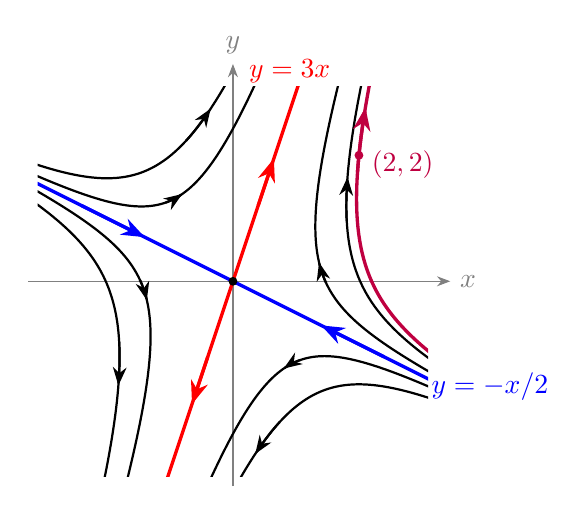
\begin{tikzpicture}[scale=.8,>=Stealth]
\phaseaxes
\begin{scope}\clip(-3.1,-3.1)rectangle(3.1,3.1);
\foreach \ca in {-.6,-.23,.23,.6}{\foreach \cb in {-.6,.6}{
\draw[orbit]plot[domain=-2:1.5,samples=180,variable=\t]
({\ca*exp(2*\t)+2*\cb*exp(-\t)},
 {3*\ca*exp(2*\t)-\cb*exp(-\t)});
% Arrow is a segment of the exact trajectory, in increasing time.
\draw[->,orbit]plot[domain=-.06:.10,samples=20,variable=\t]
({\ca*exp(2*\t)+2*\cb*exp(-\t)},
 {3*\ca*exp(2*\t)-\cb*exp(-\t)});
}}
\draw[outward](-1.1,-3.3)--(1.1,3.3);
\draw[inward](-3.3,1.65)--(3.3,-1.65);
\foreach \s in {-1,1}{
\draw[->,outward](.4*\s,1.2*\s)--(.65*\s,1.95*\s);
\draw[->,inward](2.4*\s,-1.2*\s)--(1.4*\s,-.7*\s);
}
\draw[purple,very thick]plot[domain=-2:1,samples=180,variable=\t]
({6/7*exp(2*\t)+8/7*exp(-\t)},{18/7*exp(2*\t)-4/7*exp(-\t)});
\draw[->,purple,very thick]plot[domain=-.05:.12,samples=20,variable=\t]
({6/7*exp(2*\t)+8/7*exp(-\t)},{18/7*exp(2*\t)-4/7*exp(-\t)});
\fill[purple](2,2)circle(2pt);\fill(0,0)circle(2pt);
\end{scope}
\node[purple,right]at(2.05,1.85){$(2,2)$};
\node[red,above]at(.9,3){$y=3x$};
\node[blue,below right]at(3,-1.3){$y=-x/2$};
\end{tikzpicture}\end{center}
\end{example}



%%%%%%%%%%%%%%%%%%%%%%%%%%%%%%%%%%%%%%%%%%%%%%%%%%%%%%%%%%%%%%%%%%%%%%%%
\section{Nodes}

% SIDE NOTE: 9:36 | Same procedure, different shape
% a) Draw the four inward rays first.
% b) One IC gives y=x^2, x>0.
% c) Arrows alone do not tell us which line is tangent near the origin.
% Ask: which term decays faster, e^(-t) or e^(-2t)?
\subsection{Both Eigenvalues Negative}
When two distinct real eigenvalues have the same sign, the origin is a
\textbf{node}. We again begin with the linear orbits and then study the
curves between them.
\begin{example}[5]{
For the system
\[
\mathbf{x}'=\begin{pmatrix}-1&0\\0&-2\end{pmatrix}\mathbf{x},
\]
sketch the linear orbits, find the solution with $\mathbf{x}(0)=(1,1)^T$,
and use its trajectory to complete the phase portrait.
}
The general solution is
\[
\mathbf{x}(t)=c_1e^{-t}\begin{pmatrix}1\\0\end{pmatrix}
+c_2e^{-2t}\begin{pmatrix}0\\1\end{pmatrix}.
\]
\paragraph{Step 1. Draw the linear orbits.}
The eigenvector lines are the coordinate axes. Both eigenvalues are negative,
so all four rays point toward the origin.

\paragraph{Step 2. Find one curved trajectory.}
The initial condition gives $c_1=c_2=1$, so
\[
\mathbf{x}(t)=\begin{pmatrix}e^{-t}\\e^{-2t}\end{pmatrix},
\qquad \boxed{y=x^2,\quad x>0.}
\]
The particle moves down and left along the parabola toward the origin.
It never reaches the origin at a finite time.
\begin{center}
\begin{minipage}[t]{.47\linewidth}\centering
\resizebox{.79\linewidth}{!}{\begin{tikzpicture}[>=Stealth]
\phaseaxes\noderays{-1}
\end{tikzpicture}}

\small First: four inward rays.
\end{minipage}\hfill
\begin{minipage}[t]{.47\linewidth}\centering
\resizebox{.79\linewidth}{!}{\begin{tikzpicture}[>=Stealth]
\phaseaxes\noderays{-1}
\draw[purple,very thick]plot[domain=.02:1.76,samples=80](\x,{\x*\x});
\draw[->,purple,very thick]plot[domain=1.3:.9,samples=20](\x,{\x*\x});
\fill[purple](1,1)circle(2pt)node[right]{$(1,1)$};
\end{tikzpicture}}

\small Then: one curved trajectory.
\end{minipage}
\end{center}
\paragraph{Step 3. Add curves in the other regions.}
For $c_1c_2\ne0$, eliminating $t$ gives
\[
 y=\frac{c_2}{c_1^2}x^2.
\]
Each curve stays in its region. The two halves of a parabola are separate
trajectories. Draw representative curves and orient them toward the origin.
\end{example}

% \subsection{Which Line Do the Curves Follow Near the Origin?}
% Both eigenvector lines point inward, but the curved trajectories are not
% tangent to both. We must compare the exponential rates.

% In Example 5, $e^{-2t}$ decays faster than $e^{-t}$. For a curve with both
% components present,
% \[
% \frac{y(t)}{x(t)}=\frac{c_2}{c_1}e^{-t}\longrightarrow0
% \quad\text{as }t\to\infty.
% \]
% The curves approach the origin tangent to the $x$-axis. This is the
% \textbf{slow direction}, corresponding to the eigenvalue closer to zero.
% The vertical linear orbits remain on the $y$-axis; they are not curved trajectories.

% For any node with two distinct real eigenvalues:
% \begin{itemize}
%     \item \textbf{Near the origin:} curved trajectories are tangent to the
%     eigenvector line whose eigenvalue has smaller absolute value.
%     \item \textbf{Farther away:} their directions tend toward the eigenvector
%     with larger absolute eigenvalue. This need not be a straight-line asymptote.
% \end{itemize}
% The curves need not be exact parabolas for other eigenvalues or eigenvectors.
%-------------------------------------------------------------
\subsection{Checking the Shape with a Direction Field}

For the system in Example 5,
\[
    x'=-x,\qquad y'=-2y,
\]
the velocity at a point $(x,y)$ is
\[
    \mathbf{x}'=
    \begin{pmatrix}-x\\-2y\end{pmatrix}.
\]
The direction field below helps us check the shapes
of our trajectories. The parabolic curves follow
the arrows and become tangent to the horizontal
axis as they approach the origin.

\begin{center}
%-------------------- Field alone --------------------
\begin{minipage}[t]{0.48\linewidth}
\centering
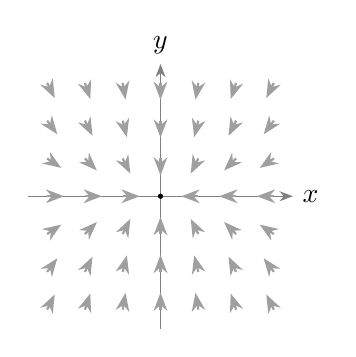
\begin{tikzpicture}[scale=0.48,>=Stealth]
    % Axes
    \draw[->,gray] (-3.5,0) -- (3.5,0)
        node[right,black] {$x$};
    \draw[->,gray] (0,-3.5) -- (0,3.5)
        node[above,black] {$y$};

    % Direction field: (-x,-2y)
    \foreach \xx in {-3,-2,-1,0,1,2,3}{
        \foreach \yy in {-3,-2,-1,0,1,2,3}{
            \pgfmathsetmacro{\mag}
                {sqrt(\xx*\xx+4*\yy*\yy)}
            \ifdim\mag pt>0pt
                \draw[->,gray!75,thick]
                    (\xx,\yy) --
                    ({\xx-0.45*\xx/\mag},
                     {\yy-0.90*\yy/\mag});
            \fi
        }
    }

    \fill (0,0) circle (2pt);
\end{tikzpicture}

\small Direction field.
\end{minipage}
\hfill
%-------------------- Field and trajectories --------------------
\begin{minipage}[t]{0.48\linewidth}
\centering
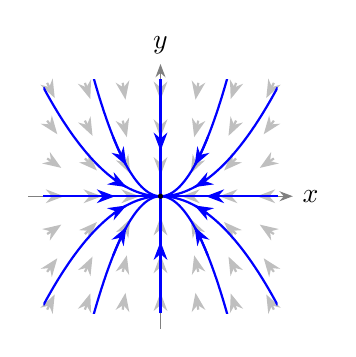
\begin{tikzpicture}[scale=0.48,>=Stealth]
    % Axes
    \draw[->,gray] (-3.5,0) -- (3.5,0)
        node[right,black] {$x$};
    \draw[->,gray] (0,-3.5) -- (0,3.5)
        node[above,black] {$y$};

    % Same direction field
    \foreach \xx in {-3,-2,-1,0,1,2,3}{
        \foreach \yy in {-3,-2,-1,0,1,2,3}{
            \pgfmathsetmacro{\mag}
                {sqrt(\xx*\xx+4*\yy*\yy)}
            \ifdim\mag pt>0pt
                \draw[->,gray!50,thick]
                    (\xx,\yy) --
                    ({\xx-0.45*\xx/\mag},
                     {\yy-0.90*\yy/\mag});
            \fi
        }
    }

    % Parabolic trajectories and inward orientation
    \begin{scope}
        \clip (-3.1,-3.1) rectangle (3.1,3.1);

        \foreach \sx in {-1,1}{
            \foreach \C in {-1,-0.3,0.3,1}{
                \draw[blue,thick,
                      domain=0.02:3.1,samples=120]
                    plot ({\sx*\x},{\C*\x*\x});

                % Decreasing |x| corresponds to increasing time
                \draw[->,blue,thick,
                      domain=1.25:0.9,samples=25]
                    plot ({\sx*\x},{\C*\x*\x});
            }
        }
    \end{scope}

    % Four linear orbits
    \draw[blue,thick] (-3.1,0) -- (3.1,0);
    \draw[blue,thick] (0,-3.1) -- (0,3.1);
    \foreach \s in {-1,1}{
        \draw[->,blue,thick] (2*\s,0) -- (1.2*\s,0);
        \draw[->,blue,thick] (0,2*\s) -- (0,1.2*\s);
    }

    \fill (0,0) circle (2pt);
\end{tikzpicture}

\small Trajectories follow the field.
\end{minipage}
\end{center}
A Matlab code that generates direction fields for $\textbf{x}'=A\textbf{x}$ will be provided on Canvas. The code may be useful for determining the shape of the solutions curves in the regions between the linear orbits.

\subsection{Classification}
% SIDE NOTE: 9:46 | Reverse time
% a) Replace the entire matrix by -A.
% b) Keep the paths; reverse all motion arrows.
% c) Same tangent rule near the origin.
Suppose we modify the system from Example 5 as follows
\[
\mathbf{x}'=\begin{pmatrix}1&0\\0&2\end{pmatrix}\mathbf{x}.
\]
Now the eigenvalues are both positive, and the general solution has the form $x=c_1e^t$ and $y=c_2e^{2t}$. Eliminating $t$ gives the same curves, but the motion is reversed. This general shape of the phase portrait always occurs whenever the eigenvalues of $A$ are real, distinct, and have the same sign. The equilibrium point $\textbf{x}^*=(0,0)$ in this case is classified as a \textbf{node}. 

Even though the solution curves have the same shape, the orientations are complete opposites. The main difference is the \textit{stability} of the equilibrium. To fully classify an equilibrium, you must state the type and stability. The attracting equilibrium on the left is called a \textbf{stable node}, and the repelling equilibrium on the right is called a \textbf{unstable node}. We will discuss this in more detail in the next lecture.

\begin{center}
\begin{minipage}[t]{.40\linewidth}\centering
\resizebox{.90\linewidth}{!}{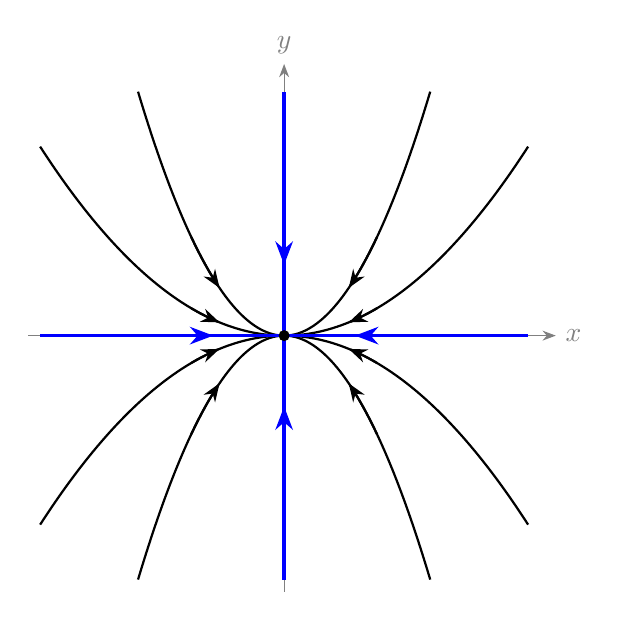
\begin{tikzpicture}[>=Stealth]
\phaseaxes\nodecurves{-1}\noderays{-1}
\end{tikzpicture}}

\small Inward: $\lambda_1=-1$, $\lambda_2=-2$.
\end{minipage}\hfill
\begin{minipage}[t]{.40\linewidth}\centering
\resizebox{.90\linewidth}{!}{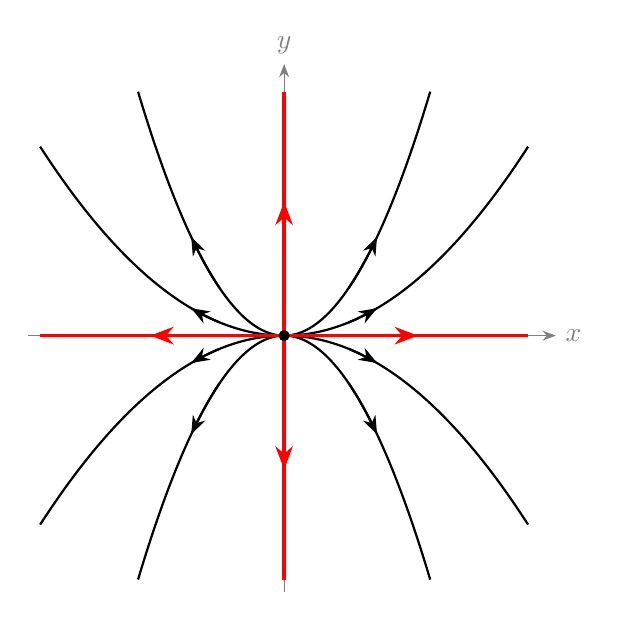
\begin{tikzpicture}[>=Stealth]
\phaseaxes\nodecurves{1}\noderays{1}
\end{tikzpicture}}

\small Outward: $\lambda_1=1$, $\lambda_2=2$.
\end{minipage}
\end{center}

\subsection{Saddles versus Nodes}
Saddles have \textbf{hyperbola-like} trajectories  $ y= \frac{C}{x}.$
Nodes have \textbf{parabola-like} trajectories  $y = Cx^2.$  We can compare them side-by-side. 
\begin{center}
%-------------------- Saddle --------------------
\begin{minipage}[t]{0.48\linewidth}
\centering
\textbf{Saddle}

\medskip
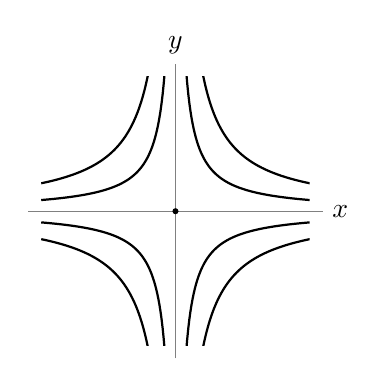
\begin{tikzpicture}[scale=0.55]
    % Coordinate axes
    \draw[gray] (-3.4,0) -- (3.4,0)
        node[right,black] {$x$};
    \draw[gray] (0,-3.4) -- (0,3.4)
        node[above,black] {$y$};

    % Curved trajectories: y=C/x
    \begin{scope}
        \clip (-3.1,-3.1) rectangle (3.1,3.1);
        \foreach \C in {-2,-0.8,0.8,2}{
            \draw[thick,domain=0.12:3.1,samples=120]
                plot (\x,{\C/\x});
            \draw[thick,domain=-3.1:-0.12,samples=120]
                plot (\x,{\C/\x});
        }
    \end{scope}
    % Equilibrium
    \fill (0,0) circle (2pt);
\end{tikzpicture}

\small
Curves move toward the origin and then bend away.
\end{minipage}
\hfill
%-------------------- Node --------------------
\begin{minipage}[t]{0.48\linewidth}
\centering
\textbf{Node}

\medskip
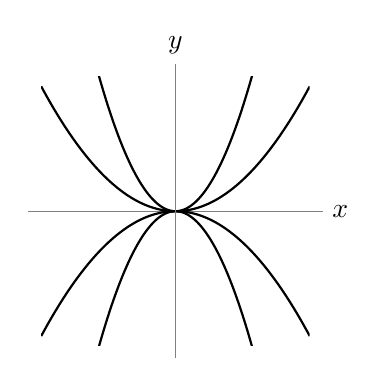
\begin{tikzpicture}[scale=0.55]
    % Coordinate axes
    \draw[gray] (-3.4,0) -- (3.4,0)
        node[right,black] {$x$};
    \draw[gray] (0,-3.4) -- (0,3.4)
        node[above,black] {$y$};

    % Curved trajectories: y=Cx^2
    % The two halves are separate trajectories.
    \begin{scope}
        \clip (-3.1,-3.1) rectangle (3.1,3.1);
        \foreach \C in {-1,-0.3,0.3,1}{
            \draw[thick,domain=0.02:3.1,samples=120]
                plot (\x,{\C*\x*\x});
            \draw[thick,domain=-3.1:-0.02,samples=120]
                plot (\x,{\C*\x*\x});
        }
    \end{scope}
\end{tikzpicture}

\small
Curves meet at the origin tangentially.
\end{minipage}
\end{center}

% In the next lecture, we will explain \textit{stability} in more detail. We will also go over how to sketch nodes in more detail. The plan for the following lectures is to cover the remaining five types of phase portraits. We will learn how to classify them based on the eigenvalues of the $A$ matrix. Each type of phase portrait has interesting features that distinguish them.  



\end{document}
